\documentclass[10pt,letterpaper]{article}
\newcommand{\tab}[1]{\hspace{.1\textwidth}\rlap{#1}}
\usepackage{calc}
\usepackage{fullpage}
\usepackage{pgfplots}
\pgfplotsset{compat=1.12}
\usepackage{graphicx}
\graphicspath{ {images/} }

\begin{document}
	\title{Math 360 Project 1: Analysis of Predator-Prey Systems}
	\author{Erica Chase}
	\date {September 21, 2015}
	\maketitle
	\section{Introduction}
		One interesting characteristic of predator-prey systems is that they are typically oscillatory as the populations of each species rise and fall. Many other factors can affect this behavior, such as environmental change, specific weather conditions, changes in available resources, disease, and genetic variation. The predator has a direct relationship with the prey; that is, as the prey population increases or decreases, the predator population follows suit. The opposite is true when starting with the predator; as the population of the predator increases, the population of the prey decreases and vice-versa.
		\newline \newline
		This can be seen in the following model, given that $x_{n}$ is representative of a population of mice, and $y_{n}$ is representative of a population of hawks.
		\newline \newline
		\centerline{$\Delta x_{n} = r_{1} x_{n} (1 - y_{n} / M_{1})$}
		\newline
		\centerline{$\Delta y_{n} = r_{2} y_{n} (1 - x_{n} / N_{1})$}
		\newline \newline
		Both $x_{n}$ and $y_{n}$ are present in both difference equations, showing they significantly affect each other. In this problem, we're going to look at a few different scenarios revolving around this predator-prey relationship model.
	\section{Parameters}
		The given problem provides a couple different guidelines for determining the parameters of the model. This includes the rate of population rise and fall and equilibrium values, defined by the given variables. 
		\begin{center}
			\begin{tabular}{c l}
				Parameter & Description \\
				\hline \hline
				$x$ & Population of mice \\
				$y$ & Population of hawks \\
				$n$ & Number of generations \\
				$r$ & Rate of population change \\
				$M$ & Limiting factor of hawk population growth\\
				$N$ & Limiting factor of mouse population growth\\
			 \end{tabular}
		\end{center}
		It's important to note some limitations on these parameters. For example, $x$ and $y$ must be positive integers because negative numbers or fractions cannot exist in a population. $n$ must also be positive because the number of generations will always be increasing. $M$ and $N$ are limiting factors, and must be larger than $x$ and $y$, respectively, to maintain a positive population. 
		\subsection{Effect of Population Rate of Change}
			The given problem asks if the population of mice grows at a 5\% rate per generation in the absence of hawks and the population of hawks falls by 6\% in the absence of mice, what can be said about the parameters in this model?
			\newline \newline
			The parameter used to represent this percent change in population growth is $r_{1}$ in the mouse population and $r_{2}$ in the hawk population. This parameter has a direct scaling effect on the rest of the model within the system; that is, as $r_{1}$ or $r_{2}$ change, the entire model is changed at the same rate, increasing or decreasing with $r$. The presence of the hawks in the mouse population, and vice-versa, are the only things stopping the populations from growing exponentially. 
		\subsection{Effect of Equilibrium Values}
			The problem also asks about the effect of equilibrium values on the parameters, specifically when there is an equilibrium when the population of mice is 200,000 and the population of hawks is 1,500.
			\newline \newline
			The parameters that have a significant effect on the equilibrium value are the $n$, the number of generations, and $M_{1}$ and $N_{1}$, the limiting factors. As $n$ increases, the populations will approach their equilibrium values. The populations are prevented from growing exponentially and forced towards their equilibrium values by $M_{1}$ and $N_{1}$.
			\newline \newline
			The given equilibrium values give us the final piece of information needed to solve for $M_{1}$ and $N_{1}$.
			\begin{center}
				\begin{tabular}{l}
					$\Delta x_{n} = r_{1} x_{n} (1 - y_{n} / M_{1})$ \\
					$\Delta y_{n} = r_{2} y_{n} (1 - x_{n} / N_{1})$ \\ \\
					$0 = 1.05 (200000) (1 - 1500 / M_{1})$ \\
					$0 = .94 (1500) (1 - 200000 / N_{1})$ \\ \\
					$M_{1} = 1500$ \\
					$N_{1} = 200000$ \\
				 \end{tabular}
			\end{center}
	\section{Long-term Behavior}
		Now that we have solved for all variables in the system, we can model the long-term behavior over generations. The problem asks for a behavior given a specific initial population, as well as the intricacies at local minimum and maximum values.
		\subsection{Given Initial Population}
			The problem gives a specific instance where the initial population of mice is 300,000 and the initial population of hawks is 1,200 and asks how the populations change over the course of at least 500 generations. 
			\newline \newline
			As the graph below shows, both populations oscillate above and below their equilibrium points. The mouse population shows a much more drastic difference due to having a much larger initial population. It's difficult to see the oscillation in the hawk population due to scaling, but the data shows that it oscillates approximately $\pm 850$ points about its equilibrium points. 
			\newline \newline
			The cycle of oscillation seems to repeat itself roughly every 120 generations. At each oscillation, the peaks appear to rise a little higher and the valleys appear to dip a little lower. I believe eventually the environment will have trouble allowing an increasingly growing population, and both the mice and hawks will either have to stabilize or begin to fall.
			\newline
			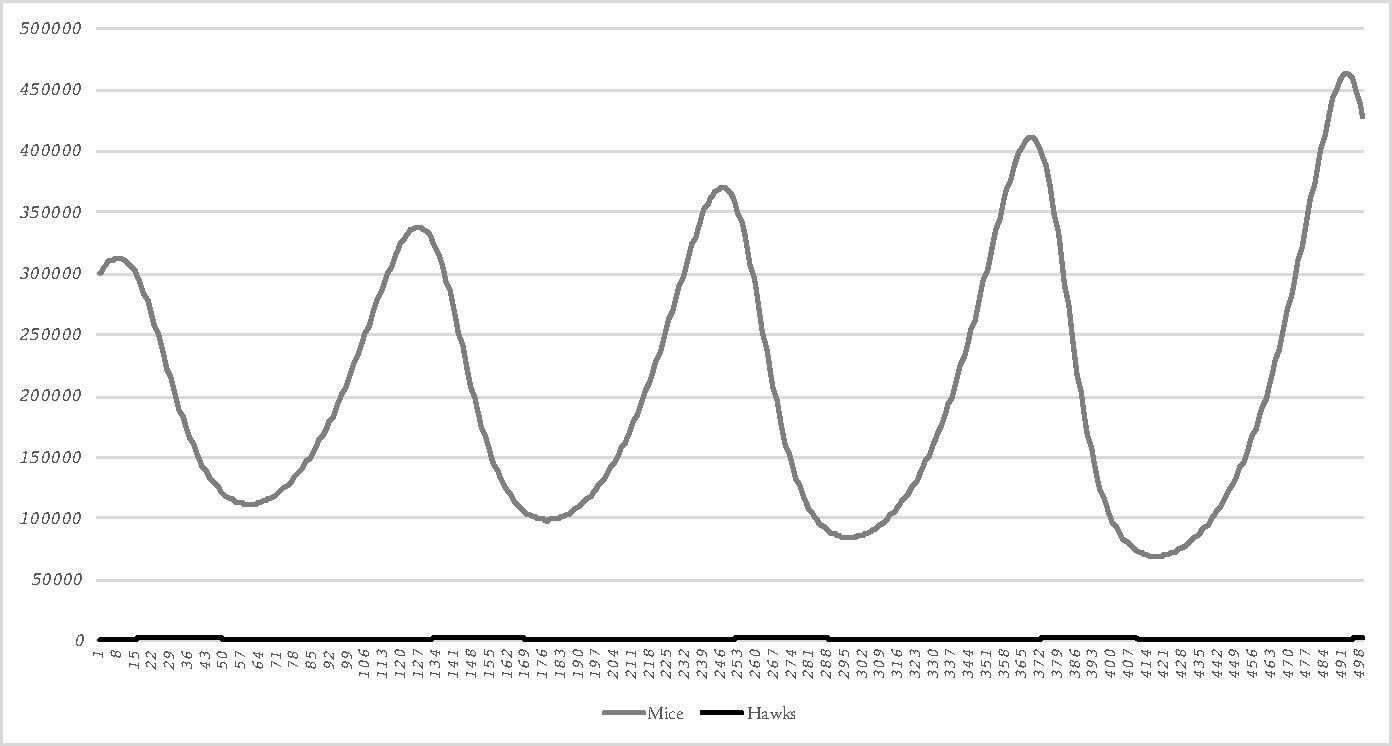
\includegraphics[width=\textwidth]{graph1.pdf}
		\subsection{Local Maximum and Minimum Population Values}
			Additionally, the problem asks about the population of hawks when the mice are at their maximum and minimum values, and vice versa. As shown in the above graph, when the mice are at their local peak population, roughly 300,000-450,000, the population of hawks begins to rise. When the mice population is at its lowest, between approximately 75,000 and 100,000, the hawk population begins to fall. And inverse relationship can be seen when starting with the mouse population. When the hawk population peaks, the mouse population falls. When the hawk population is at its lowest, the mouse population rises. This graph intuitively matches the expected behavior; that is, as the population of the hawks rise, they need to eat more mice, and thus the population of mice fall. As the population of hawks fall, the population of mice has room to grow. Because these behaviors affect each other, an oscillation is seen.
	\section{Further Exploration}
		There are many facets of this problem to explore, especially with so many variable and situations. These include changes in growth rates, alternative initial values, and environmental changes. 
		\subsection{Random-Valued Rate Parameters}
			One specific factor the problem addresses is that of random-valued rates, i.e. what would happen if the rate of growth changed slightly over each generation? This can be modeled below, where the value of $r_{1}$ and $r_{2}$ was randomly generated for each generation.
			\newline
			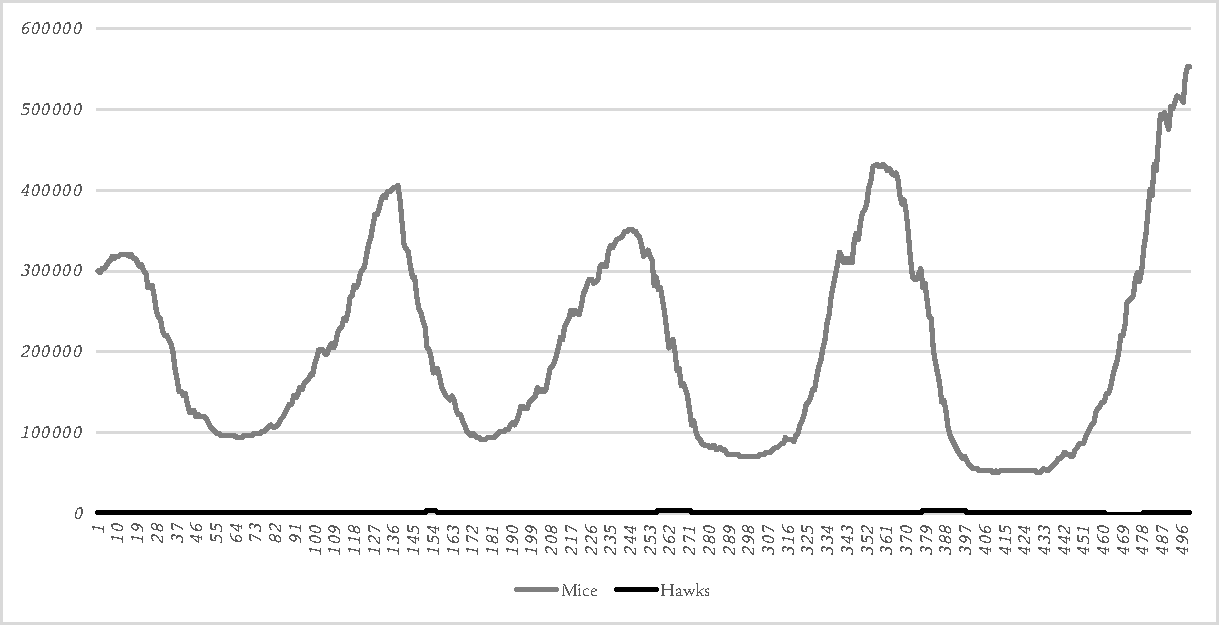
\includegraphics[width=\textwidth]{graph2.pdf}
			\newline 
			The above graph illustrates that while the rates are constantly changing, the overall oscillatory effect does not change. The hawk population will still rise as the mouse population does and the mouse population will still fall as the hawk population rises. The reveals a major trend in general animal behavior. Growth rates are likely to rise and fall each generation based on a huge number of factors, but large amounts of hawks will still need to eat large amounts of mice, and large amounts of mice can only thrive if they're not being eaten by hawks. 
		\subsection{Change in Initial Population}
			Another factor the problem asks us to consider is that of alternate initial population values. For example, what if the initial mouse population was 150,000 and the initial hawk population was 1,600? This is shown in the graph below:
			\newline \newline 
			\centerline{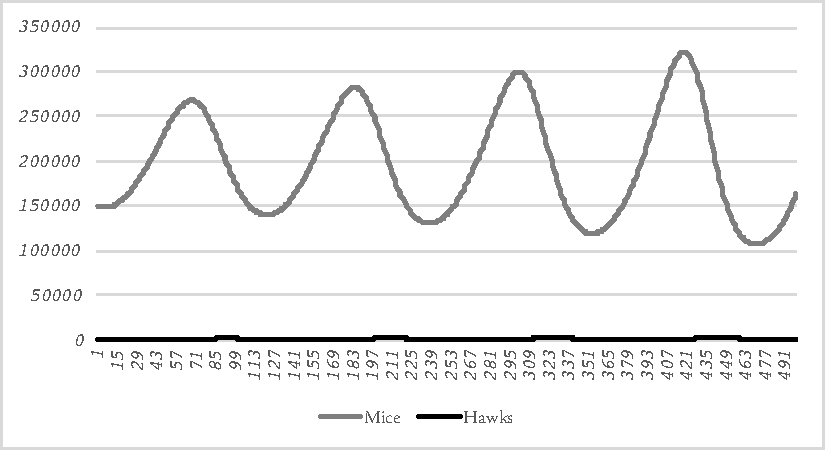
\includegraphics{graph3.pdf}}
			\newline \newline 
			No major changes seem to occur. The pattern of oscillation is the same, occurring every 120 years and rising and falling a little more each year. The populations also still seem to hover around the given equilibrium values. The biggest change is that, within 500 iterations, the overall populations don't seem to rise and fall as much as they did in when the initial populations for mice and hawks were 300,000 and 1,200, respectively.
		\subsection{Added Limiting Factors}
			The predator-prey relationship isn't the only factor limiting the growth of the mouse and hawk populations. In general, there is no existing environment capable of supporting an increasingly growing population. We saw in the above graphs that the populations were increasing after each oscillation cycle, and that cannot be supported long-term. Because of this, we add additional limiting factors that account for things like climate, resource saturation, disease, and a number of other things. We call these new limiting factors $N_{2}$ and $M_{2}$ and add them to the given model:
			\newline \newline
			\centerline{$\Delta x_{n} = r_{1} x_{n} (1 - y_{n} / M_{1}) (1 - x_{n} / N_{2})$}
			\newline
			\centerline{$\Delta y_{n} = r_{2} y_{n} (1 - x_{n} / N_{1}) (1 - y_{n} / M_{2})$}
			\newline \newline
			The problem notes that $N_{1}$ should be less than $N_{2}$ and that $M_{1}$ should be less than $M_{2}$. This makes sense because the environmental and non-predator/prey values should have a much larger effect on the overall population growth. In a normal non-predator/prey population model without a limiting factor, you're likely to see exponential growth until resources run out, and this added limiting factor accounts for that. 
			\newline \newline
			Next, we are to take $N_{2} = 400000$ and $M_{2} = 3500$ and use those values in a few previous scenarios. First, let the initial population of mice be 300,000 and the initial population of hawks be 1,200. With the new model, we get the graph below:
			\newline \newline \newline
			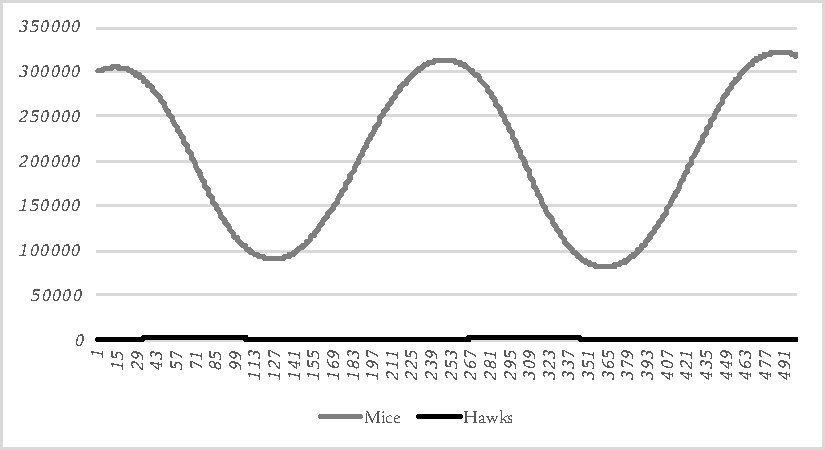
\includegraphics[width=\textwidth]{graph4.pdf}
			\newline \newline
			Intuitively, this graph makes a lot of sense with the added limiting factors. As the oscillation cycle repeats, the peaks and valleys rise and fall, respectively, at a much slower rate. Additionally, the cycle repeats itself after about 250 generations, over twice long as it was repeating before. The equilibrium values remain the same. The local maximum and minimum values also appear to behave in the same way they did before. 
			\newline \newline
			Let's test the new model with the change in initial population from before, where the mice population started at 150,000 and the hawk population started at 1,600.
			\newline \newline 
			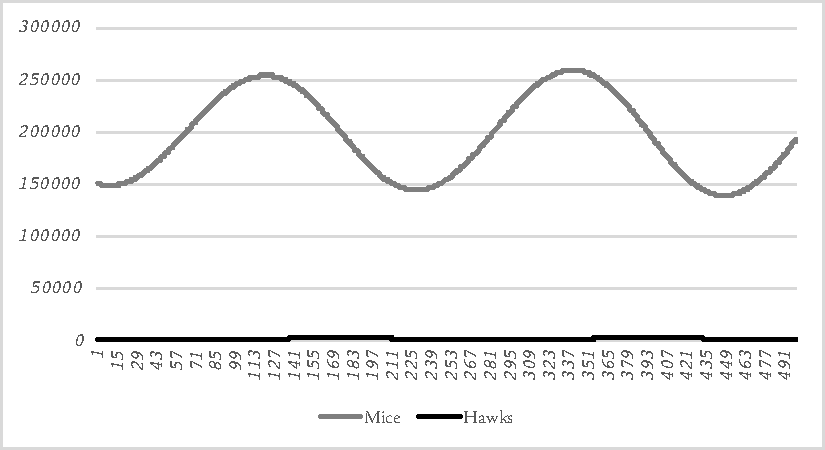
\includegraphics[width=\textwidth]{graph5.pdf}
			\newline \newline
			This changes the overall range of the graph; the peaks and valleys don't rise and fall as much as they had previously and the cycle oscillates much more slowly. However, the populations seem much more stable, as the second limiting factor prevents them from growing above their means. 
			\newline \newline
			What would happen if we force initial values above their limiting factors? For example, what if we began with a mouse population of 600,000 and a hawk population of 5,000? We know that these are larger than the limiting factors previously given, and thus should not correctly fit the model.
			\newline \newline 
			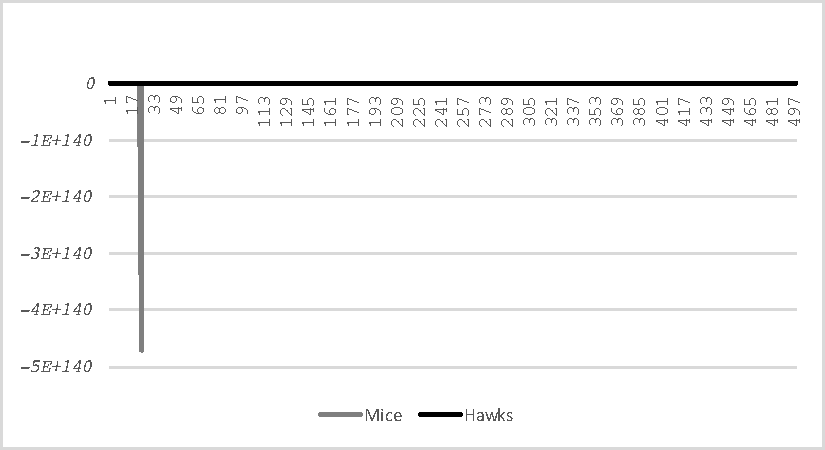
\includegraphics[width=\textwidth]{graph6.pdf}
			\newline \newline
			This idea completely breaks the model, as the mouse population shows one extreme dip and then both populations can't even display a value after about 26 points. This shows how important the limiting factors are to the model to maintain any kind of stability or structure. 
		\subsection{Changes in Environment}
			As stated before, the additional limiting factors in the model account for things outside the predator-prey system, such as disease, climate, hunting, etc. In order to further illustrate this idea, let's add one weird dude who lives in the woods. This guy, we’ll call him Steve, had aspirations of being a successful surgeon since he was very very young. Steve put all of his time, money, and effort into medical school trying to be the best surgeon in the world. Unfortunately, Steve is an idiot. Steve drops out of medical school, and, now that he's poor, has to reside in a cave in the woods. Steve is a trooper though, and Steve's dreams never died. Now Steve routinely catches 15\% of the mice in every new generation to use in sketchy back-woods experiments. No one knows what Steve is trying to accomplish, but those mice are taken out of the population in the altered predator-prey model.
			\newline \newline
			Let's see how this affects the model:
			\begin{center}
				\begin{tabular}{l}
					$\Delta x_{n} = 1.05 x_{n} (1 - y_{n} / 1500) (1 - x_{n} / 400000) - .15 x_{n}$ \\
					$\Delta y_{n} = .94 y_{n} (1 - x_{n} / 200000) (1 - y_{n} / 3500)$ \\
				 \end{tabular}
			\end{center}
			This shows that for every new generation, an \emph{additional} 15\% of the mouse population is removed. The long-term behavior of this can be seen in the graph below, with an initial mouse population of 300,000 and a hawk population of 1,200:
			\newline \newline 
			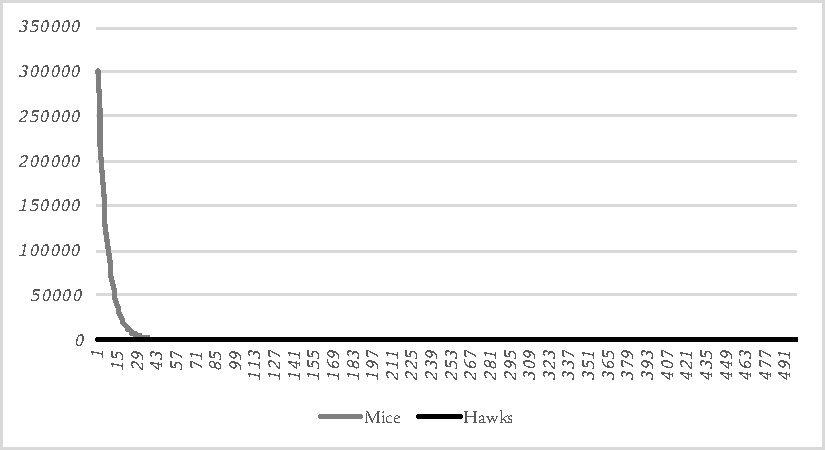
\includegraphics[width=\textwidth]{graph7.pdf}
			\newline \newline
			Turns out it only took about 120 generations for Steve to cause the entire mouse population to go extinct. Now, the hawks have nothing to eat and they're not happy about it. By the time the mice go extinct, there are about 5 hawks left contemplating eating Steve out of anger and starvation. If the angry hawks eat Steve, we can expect a small rise in hawk population around the 120th generation, and then it will quickly drop to 0. Steve leaves his family with a massive amount of debt from his student loans. 
	\section{Conclusions}
		Many conclusions can be drawn from the exploration of this problem. First, we took a look at how the different parameters affect the model, and saw that the rate, $r$, had a direct scaling effect on the model. Later we saw that even randomized values of $r$ didn't change the overall behavior of the model. This shows that ultimately the nature of the animals will change slightly from one generation to the next as environmental factors take place, but overall the animals will behave in a standard way. 
		\newline \newline
		Next, we saw how the equilibrium values affected the model. In the unaltered original model, the equilibrium served as the limiting factor for the opposing species, or $M_{1}$ and $N_{1}$. Later, secondary $M$ and $N$ values were added to serve as an additional limiting factor, typically due to land mass and available resources. 
		\newline \newline
		Then we observed long-term behaviors of the model as we changed certain factors. For example, changing the initial population values kept the model roughly the same, exhibiting only small changes in the peaks and valleys of the graphed data. Other values, such as the frequency, period, and equilibrium stayed the same, demonstrating the stability of the model.
		\newline \newline
		Adding additional limiting factors dramatically altered the data in a very realistic way. Before $M_{2}$ and $N_{2}$ were added, nothing was taking exponential population growth into account, and so the populations would increase by a fairly large amount every 120 generations or so. Adding these second limiting factors doubled the period of the graph and drastically lowered how much the population increased each cycle. In real life, populations tend to plateau after their needs are satisfied, and, combined with the oscillation of the predator-prey system, this addition fits that idea.
		\newline \newline
		These new limiting factors made it possible to completely break the model simply by exceeding the value of the limiting factors. This was important because it showed the value of adequate resources for a certain population, and having more population than resources simply cannot sustain itself. 
		\newline \newline
		Finally, outside factors were taken into consideration, such as the addition of a person removing part of the population each generation. This caused the population to go extinct extremely quickly and showed how huge of an impact outside factors can have on a population.
\end{document}

